\documentclass[11pt]{article}
\title{%
Skeleton of final report\\\large
\color{white} blank line\\
\color{black}
COMS3\\
Group 9\\
Tracking Interconnected Twitter Links\\
Using Graph Database Neo4j}
\date{2017}
\author{Lindiwe, Clifford, Thomas}

\usepackage[margin=1.5in]{geometry}
\usepackage{hyperref}
\usepackage{graphicx}
\hypersetup{
    colorlinks=true,
    linkcolor=blue,
    filecolor=magenta,      
    urlcolor=blue,
}

\begin{document}
\maketitle
\pagenumbering{gobble}
\newpage
\tableofcontents
\newpage
\pagenumbering{arabic}
\section{Introduction}
\subsection{Overview}
This purpose of this project is to graph Twitter data so that hidden trends and patterns may be revealed.
\subsection{Neo4j}
Neo4j is the leading graphic database management system, that distinguishes itself from other systems through its ease of use and its speed. Its was initially launched in 2010. Its fundamental design is to store data as nodes, edges and attributes. Nodes are connected by edges, both can have any number of attributes.
\subsection{requirements}
To run the code as desired the following programs or packages are required
Neo4j v3.2.4\newline
Python v2.7.13\newline
PyCharm 2017.2.3\newline
TextBlob v0.13.0\newline
Tweepy v3.6.0\newline
py2neo v3.1.2\newline
$\href{https://github.com/TJ721988/SEgroup9/blob/master/Cipher_Queries.txt}{Cipher Queries} (GitHub)\newline 
\href{https://github.com/TJ721988/SEgroup9/blob/master/Twitter_neo%20_final.py}{Twitter neo final} (GitHub)\newline $
\subsection{Running the code}
The specifics of running the code as desired can be found on $\href{https://github.com/TJ721988/SEgroup9/blob/master/README.md}{\texttt{GitHub in the ReadMe}}$  document
\section{Description}
We import public data from twitter and store it in a Neo4j database. This database is graphically represented through the Neo4j Browser, which shows nodes and connections, in different colours and sizes to highlight and differentiate various things. Filters can be applied to customise or limit what the graph shows. For example only tweets with a certain phrase or hashtag, "\#neo4j", can be shown. This can give an idea about the age, location or gender of people tweeting about Neo4j.


\begin{figure}
\subsection{Design}
Figure 1 shows a demo of the final look.\newline
 Green nodes are people on twitter, labelled by their twitter handle, they share an edge labelled "created by" to red nodes, labelled "T", with anything they tweet. Should anyone retweet this tweet, then a "RT" node is created in purple, sharing "created by" edges with the original tweet and the retweter. A blue node is created in a similar fashion, when someone replies to or mentions someone else on Twitter.\newline
 The purple node in the center is the topic we chose to filter the tweets through. We thought "Trump" should always be trending, although in different volumes, based on the time of day. The central topic shares an edge withh all shows tweet, labelled "generated by". \newline
Every time the python script is run it increases the database size, the figure below was created after running the code just once. Twitter limits what we can access, running the script again an hour later brings in a similar quantity of data. 
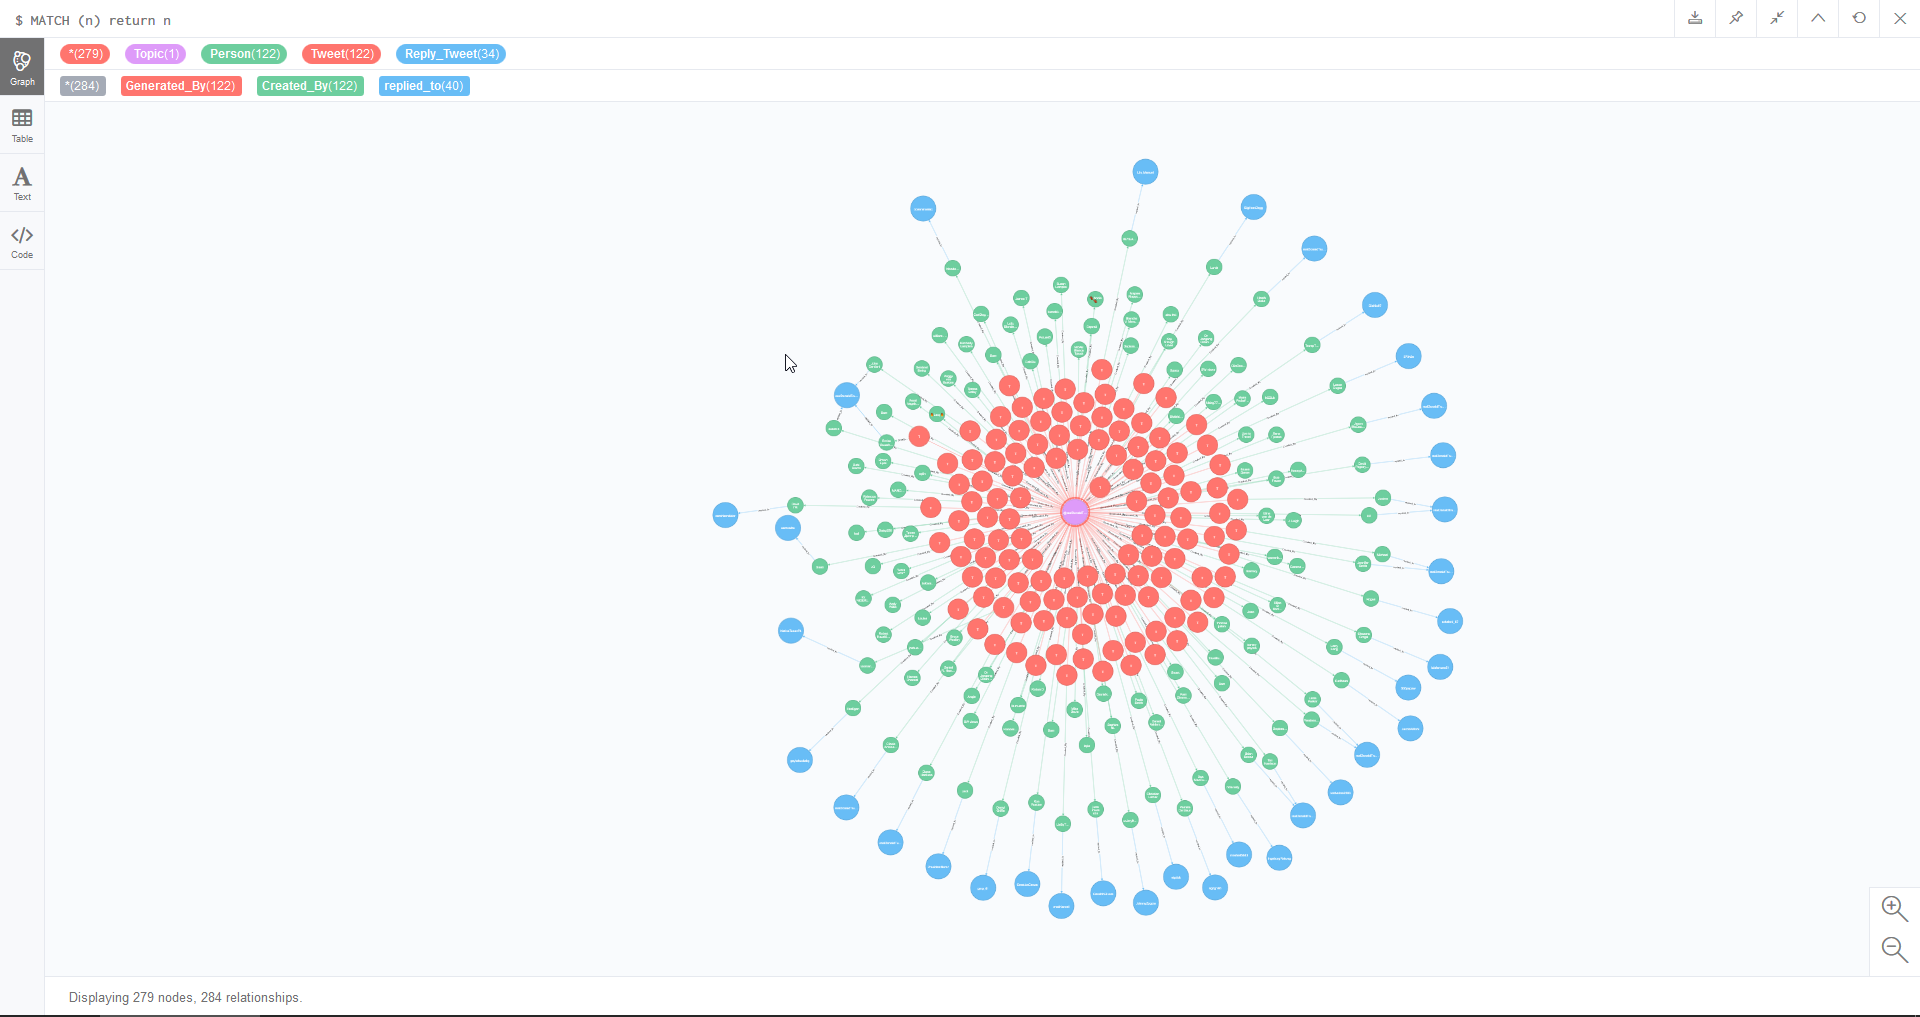
\includegraphics[width=\textwidth]{Neo2}
\caption{Neo4j Browser look} 
\label{fig: 1}
\end{figure}

\begin{figure}
Figure 2 shows the data process, from Twitter to the final front-end interface.\newline
\newline
\includegraphics[width=8cm]{Flow}\newline
\caption{Data process} 
\label{fig: 2}
The Tweepy API collects data from the continuous flow of information that is Twitter, and converts it to a JSON string. This string is then processed to neo4j data and analysed by TextBlob. The data is then passed to Neo4j, where it is stored and displayed as a graph. The graph can be manipulated and filtered through the Neo4j Browser
\end{figure}

\begin{figure}
Figure 3 shows the basic idea behind the set up of the database.\newline
\includegraphics[width=8cm]{Graph}\newline
\caption{Neo4j database set up} 
\label{fig: 3}
Our nodes are people, tweets, retweets, replies and the central topic, they have various properties, such as age, gender, sex (where appropriate), time created, location.
The edges "generated by", "created by" and "replied to" link the nodes. Edges can have properties too, properties not only provide additional information, that can be seen by clicking or hovering over a node/edge, they also can be used as filters to search/limit the data.
\end{figure}

\begin{figure}
To emphasize how Neo4j simplifies the data being worked with to a graph Figure 4 shows the JSON string, the raw information, and the equivalent graph.\newline
\includegraphics[width=15cm]{JSON}\newline
\caption{Raw data vs graph} 
\label{fig: 4}
The graph is a better presentation, that offers a better overview and logical structure of interconnections. This is mainly because it is easy to look at a graph showing the connection, than trying to imagine it for oneself.\newline
Additionally the graph shows a lot less information at the first glance, data not relevant to the connection network aren't shown in the overview, but can easily be accessed by selecting a node/edge. The viewer can choose what information he wants, and doesn't need to sift through lines and lines of text.
\end{figure}

The JSON for "Wonderfulvideo2" isn't shown, as itis very similar to that of "FightinFourteen", which in contained in the second set of bracket{}.
Details such as friends, followers and time aren't shown on the graph, but hovering over an element, or selecting it, will reveal these an other properties.
\newline
We discussed including the location of where the tweet was made, however this is problematic for several reasons
\begin{itemize}
\item Not all users share their location with twitter
\item Location isn't always accurate
\item Different providers share locations differently (3 locations from our testing include, "\#GameofThrones", "Basin, WY, United States", "Kenya")
\end{itemize}
In the end we left the location as a property of the nodes, which means it can be used as a filter. However further analysis of the location into a uniformed method would have to be applied for this information to be fully utilised.\newline

Using a text analysis tool (TextBlob) we can look at the content of a tweet to see whether it's an opinion. We can also look at the sentiment of the content to determine whether a tweet is positive or negative. These are stored as properties which again can be used as filters, showing only tweets that are positive opinions, or no opinions at all...

\subsection{Back-end}
The back-end of the project imports data from Twitter to python as a JSON stream. The JSON is then analysed and converted to neo4j data. In the process Nodes and edges are created and properties are assigned. External analysis such as sentiment are done before the conversion to neo4j, and passed along as properties.
We don't have a server to host the Neo4j data, which means that when a different machine runs the code they will collect seperate data from twitter, based on what is trending at the time. This can result in differences based on when and how often Twitter data is collected, however by using a topic like "trump" we hope to always have a fair amount of hits.\newline

\subsection{Front-end}
The front end interface is the Neo4j browser. Unfortunately we don't have a server to host this, so system settings can't be saved, such as the graphic template for colour, size and the like. This also means that changes to the data being viewed are done as Cipher queries. The browser itself allows for movement of nodes, zooming and inspection of elements as well as style changes, all of which can be done from the tool bar around the view panel. Editing the edges, requires a node to be selected and the "Expand child relationships" to be toggled, around the node. Properties of individual nodes can been viewed by hovering over a node, or selecting it and viewing either the table or text views, from the tool bar on the left.

\subsection{application}
The Neo4j database system is nice to look at and fun to play around with, beyond that it has real world applications. These applications are manifold and extend beyond just Twitter data. As we looked at Twitter data, lets look at how this data can analysed. We can track frequency of which people tweet about a topic based on the time of day. We can look at what a certain age/race/gender typically tweets, what sentiment it has, and how many retweets it gets. A company could see how many and what kind of person is tweeting about their product. The negative sentiment filter can be applied to only show people complaining about the product, to address community issues.

The hope is that the above queries and other similar ones will reveal hidden patters, once such pattern have been identified algorithms and further filters can be created to analyse these patterns are try find more. One of these hidden patterns was profiling, which a lot of online websites use when recommending you anything or showing you adverts. 

\subsection{looking forward}
The first improvement we would like to make would be to host the Neo4j database on a server, so that visual designs and templates can be stored for a uniform look. This also means that there would be a uniform database for users to use, and not a custom generated one based on the time of the execution. The next would be a script, either through a website or a program to automate the initial set up in Python, so that the user just needs to select his preferences or enter a topic into a search field and the script does the rest and displays the results in the browser. This could also eliminate having to run Cipher queries manually, as the script would take care of that, the user just needs to select his preferences and hit update.

\section{Members}
who did what




\end{document}